% Changed: recover service economics, complementary breadth and mechanism-led evaluation.
% Protected: all measurement clocks, cohort distinctions and negative outcomes.
% Meaning-Check: PRESERVED
% Risk-Flags: none
\section{Evaluation}
\label{sec:evaluation}
We test whether governing layout, evidence and publication creates useful shared service state: first complete-cost performance, then behavior, governance and operating conditions.

\begin{figure*}[t]
\centering
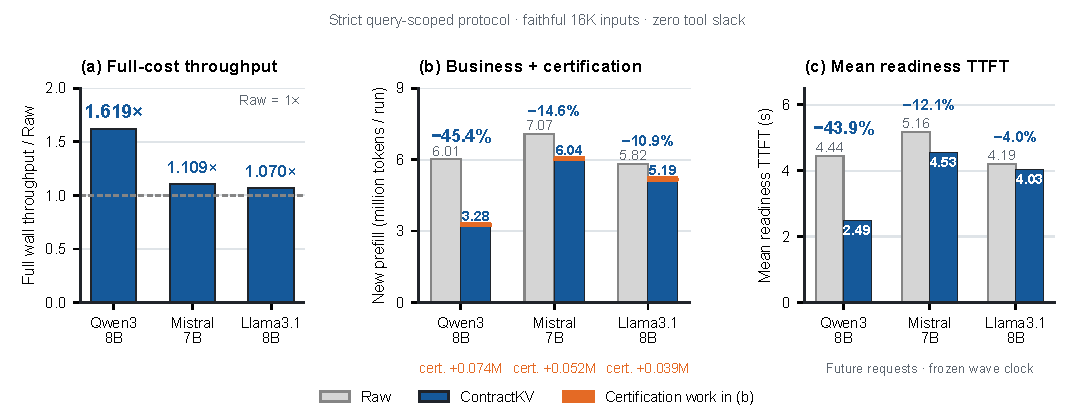
\includegraphics[width=\textwidth]{figures/fig2_full_cost_benefits.pdf}
\caption{Strict query-qualified performance on six source-disjoint HotpotQA/RepoBench templates, three processes/model, faithful 16K inputs, and zero slack. (a) Throughput charges all business responses, qualification, failed attempts, and synchronous waiting. (b) Actual business plus qualification new-prefill counts per run; orange caps mark certification work at its true scale, with exact added counts below. (c) Mean readiness TTFT over future requests uses the frozen two-request wave clock. Three-repeat values and tail statistics are reported separately.}
\label{fig:performance}
\end{figure*}

\subsection{Workloads, Controls, and Units}
\label{sec:protocol}
The primary cohort contains three HotpotQA and three RepoBench sources, chosen by frozen hash order after excluding 567 previously used sources~\cite{hotpotqa2018,repobench2024}. Reading-comprehension data come from the LongBench collections~\cite{longbench2024}. Each source defines a ten-tenant, ten-round template with three recurring query wrappers and changing private metadata. This is an explicitly repeated authorized directory, not a measured production query distribution.

We run Qwen3-8B, Mistral-7B-Instruct-v0.3, and Llama-3.1-8B-Instruct~\cite{qwen32025,mistral2023,llama32024}. Both policies have the same 16K window, retained task content, greedy decoding, fixed seed, request order, and two-request wave clock. HotpotQA has a 128-token generation budget and RepoBench 384. \emph{Raw} retains the original order with native APC; \emph{ContractKV} uses the frozen candidate, eligibility, margin/EOS checks, and publication path. Mistral and Llama inherit the development-frozen RepoBench L0 route.

Three fresh processes/model/policy yield 10,800 business generations and 4,860 future pairs: 600 business requests/run, including 540 future requests. Six sources are the independent content units; tenant, round and process observations remain nested. Ranges are process min--max; intervals resample source clusters and repetitions.

We retain prompt/output IDs, task scores, routes, qualifications, timing, and cache counters. QA uses the frozen token-F1 scorer; code uses the existing SequenceMatcher-based edit-similarity adapter. These are declared benchmark adaptations. Material score changes use $|\Delta s|>0.03$; exact ID agreement is measured separately. The supplement gives all six sources' utility, compiled coverage and paired tails, plus process values and clock definitions.

\subsection{Does Governed Reuse Repay Qualification?}
\label{sec:mainresults}
We expect a net gain when enough admitted requests reuse a stable prefix to repay first-use qualification. Figure~\ref{fig:performance} tests this on the same source set, with no tool slack and successful and failed attempts included. Throughput improves by 1.619$\times$ on Qwen, 1.109$\times$ on Mistral, and 1.070$\times$ on Llama. The process ranges are 1.615--1.623$\times$, 1.107--1.110$\times$, and 1.068--1.072$\times$. These are complete service gains rather than prefill-only estimates.



Figure~\ref{fig:performance}(b) measures the work saved: including qualification, total new-prefill counts fall by 45.44\%, 14.64\%, and 10.89\%. These scheduler observations are workload counts, not inferred GPU time. Directly measured mean readiness falls by 43.87\%, 12.09\%, and 3.99\%.

\begin{table}[t]
\centering\small
\caption{Tail cost and admitted coverage in the primary cohort. Readiness statistics concern future requests. Full process ranges and source-cluster intervals are in the supplement.}
\label{tab:primary}
\begin{tabular}{@{}lrr@{}}
\toprule
Model & Compiled / future pairs & p99 raw $\rightarrow$ CKV (ms)\\
\midrule
Qwen & 684 / 1,620 & 8,561.8 $\rightarrow$ 9,146.6\\
Mistral & 342 / 1,620 & 9,418.2 $\rightarrow$ 9,511.3\\
Llama & 270 / 1,620 & 7,851.3 $\rightarrow$ 7,905.7\\
\bottomrule
\end{tabular}
\end{table}

The throughput result does not imply lower tails. All p99 point estimates increase (Table~\ref{tab:primary}); Mistral's source-cluster/repetition interval for p99 reduction is wholly negative, [-60.576, -0.137]\%. Mean reduction intervals are [5.640, 79.479]\%, [-0.350, 34.781]\%, and [1.550, 5.724]\%. The cohort therefore supports a full-cost execution benefit with source-dependent latency effects.

A second independent six-source Qwen cohort reaches 1.803$\times$ throughput (process range 1.798--1.808$\times$) with 774/1,620 compiled future pairs. Its results remain separate from Fig.~\ref{fig:performance}.

\noindent\emph{Finding:} admitted prefix reuse repays qualification in the task-preserving zero-slack cohort, with directly observed reductions in prefill work and complete service time.

\paragraph{Breadth across deployment configurations.}
Table~\ref{tab:deployment-width} complements the task-preserving result with four deployment configurations. The recorded 29.41--44.69\% TTFT band uses 2-s/6-s residual slack. A frozen-input, three-repeat replay charges the complete controller with zero slack and measures service wall directly. Qwen3-14B TP2 retains a 20.93\% full-cost TTFT reduction and 1.109$\times$ wall throughput; Mistral measures 0.994$\times$. Qualification therefore needs sufficient authorized reuse to repay its complete cost. All attempted and aborted work is charged.
\begin{table}[t]
\centering\footnotesize
\setlength{\tabcolsep}{3.0pt}
\caption{Four deployment configurations: recorded residual-slack accounting and a frozen-input, three-repeat complete-cost replay. \emph{Recorded} mean-TTFT reductions use the original residual-verifier convention (2-s slack; Llama 6 s). \emph{Full} charges measured complete Controller cost with zero slack; \emph{wall} is direct full-service wall (raw/CKV). Each replay uses a fresh server process; recorded and replayed columns retain their own clocks.}
\label{tab:deployment-width}
\begin{tabular}{@{}lrrrr@{}}
\toprule
Configuration & \shortstack{Recorded\\TTFT $\downarrow$} & \shortstack{Full-cost\\TTFT $\downarrow$} & \shortstack{Direct\\wall $\times$} & \shortstack{Recorded\\prefill $\downarrow$}\\
\midrule
Qwen3-8B & 37.81\% & 10.82\% & 1.020 & 59.13\%\\
Qwen3-14B TP2 & 44.69\% & 20.93\% & 1.109 & 60.57\%\\
Mistral-7B & 31.72\% & 2.00\% & 0.994 & 39.46\%\\
Llama-3.1-8B & 29.41\% & $-0.20$\% & 1.012 & 30.97\%\\
\bottomrule
\end{tabular}
\end{table}


\subsection{Does Qualification Preserve Observed Behavior?}
\label{sec:quality}
Compilation must obtain its gain within the admitted behavioral scope. Figure~\ref{fig:behavior} reports both scope coverage and free-running evidence. All 1,296 compiled future pairs have identical output IDs and unchanged scores. Including initial business rounds gives 1,440 compiled pairs with the same outcome. HotpotQA contributes compiled requests for every model; Qwen additionally admits RepoBench, whereas Mistral/Llama keep the inherited L0 route.

\begin{figure}[!t]
\centering
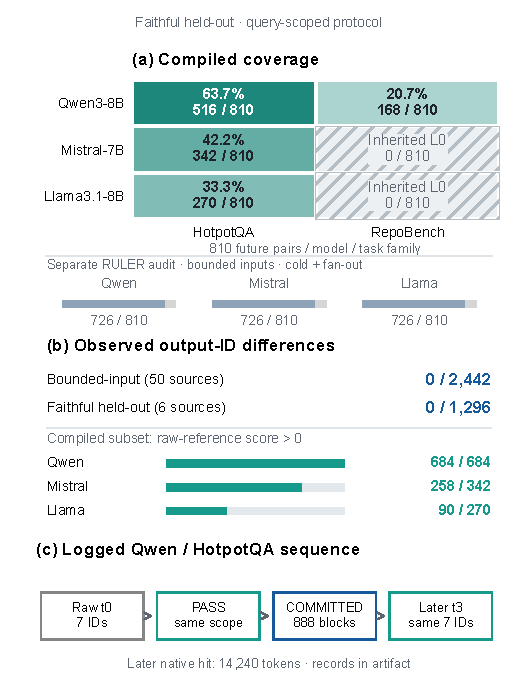
\includegraphics[width=\columnwidth]{figures/fig3_coverage_and_fidelity.pdf}
\caption{Qualification coverage and free-running evidence. (a) Each model/task cell has 810 future pairs; hatched cells inherit L0. The separate RULER strip uses bounded inputs and pooled cold/fan-out traces, not the faithful matrix protocol. (b) Output-ID differences and raw-reference positive-score counts within compiled subsets. Positive credit is not complete correctness. (c) One logged Qwen/HotpotQA witness, PASS, committed prefix and later identical output; full records are archived.}
\label{fig:behavior}
\end{figure}

Behavioral preservation and absolute utility remain different outcomes. Qwen's 684 admitted raw references all receive positive score credit; the counts are 258/342 for Mistral and 90/270 for Llama. Llama preserves 180 zero-F1 future references from two HotpotQA sources, and Mistral preserves 84 from one source. Neither exact agreement nor positive partial credit establishes semantic correctness.

All-route material increases/decreases are 0/0, 2/1 and 5/3 for Qwen/Mistral/Llama, all on L0. Scheduled raw-only repeats contain corresponding output variants, showing background variation while leaving policy-associated execution effects unresolved.

The separate 50-source bounded-input audit retains 2,442 compiled future pairs: 2,178 RULER, 174 NarrativeQA and 90 RepoBench~\cite{ruler2024,narrativeqa2018,qasper2021}, with zero compiled ID changes and 33 all-route decreases on L0. Each model's RULER coverage is 726/810 (210/270 cold, 516/540 fan-out). Figure~\ref{fig:behavior} separates this fixed-cap, mixed cold/fan-out protocol from the faithful non-RULER matrix.

\paragraph{Why the scope matters.}
A broad-wrapper development protocol admitted later wrappers and produced 108 material decreases among 3,672 compiled pairs. A Qwen NarrativeQA development case changed its raw answer under an allowed turn-field change while the compiled answer retained the witness, despite a 0.40625 candidate margin. The evaluated eligibility class was frozen before the independent sources were opened. A margin alone cannot justify extending evidence to unseen dynamic inputs.

\paragraph{Actual output horizon.}
Separate conditions produce and verify naturally terminated outputs of 642 tokens for Qwen, 769 for Mistral, and 578 for Llama, each with six correct future pairs across three processes. They use explicitly declared 128/128/192-item schemas. Llama's 224-item condition omits the final 100 items and remains a task failure. These results establish actual 512+ output conditions, not universal long-output correctness.

A common-scope HotpotQA study uses the same 30 sessions across three models and three repetitions, yielding 2,430 future pairs. Business new-prefill reductions are 48.05\%, 40.69\% and 38.38\% for Qwen, Mistral and Llama. Its zero-slack macro mean TTFT reduction is 5.242\% (source-cluster 95\% interval [$-2.162$, $12.564$]\%); the supplement gives the timing variants and the original RULER statistical analysis.

\noindent\emph{Finding:} qualified reuse preserves observed free-running behavior on admitted requests across synthetic and non-RULER tasks; coverage and reference utility identify the scope of that evidence.

\subsection{Does Governance Preserve the Service Benefit?}
\label{sec:ablation}
Figure~\ref{fig:governance} isolates governance from layout opportunity. D1 uses a prequalified layout without online registration; D2 adds verification and transactional registration. At the same 500-ms SLO, native D0, D1 and D2 deliver 0.066, 1.472 and 1.428 requests/s. D2 retains 97.0\% of D1 goodput, paying 0.044 requests/s (3.0\%) for governance; TTFTs are 194.95/194.72 ms. D0 supplies context and D1 the layout-matched comparison.

\begin{figure}[!t]
\centering
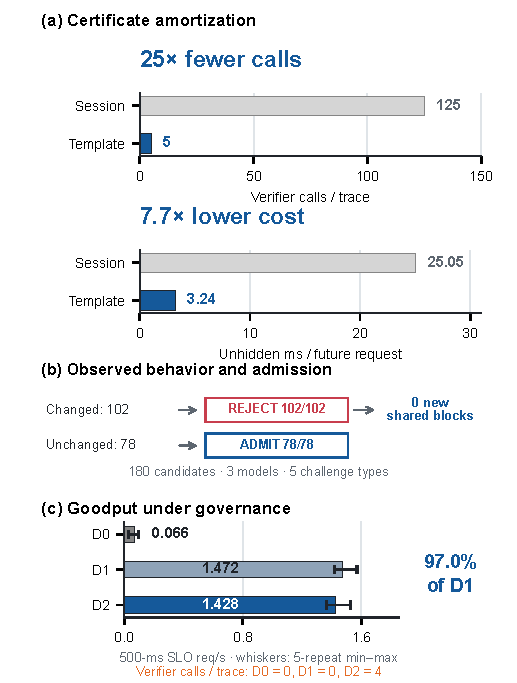
\includegraphics[width=\columnwidth]{figures/fig4_transaction_and_amortization.pdf}
\caption{Separate deployment controls. (a) Registration granularity with fixed layout/locality; three processes and 1,125 future requests/trace. (b) Three models and five challenge types: all 102 behavior-changing candidates are rejected; all 78 unchanged candidates are admitted; rejected candidates add zero shared candidate blocks. (c) Same-engine D0/D1/D2 500-ms SLO goodput; whiskers are five-process min--max, not confidence intervals.}
\label{fig:governance}
\end{figure}

\noindent\textbf{The value of admission.} In the independent three-model, five-challenge study, 102 of 180 dependency-valid candidates change free-running output IDs or termination; all 102 are rejected. The remaining 78 unchanged candidates are admitted, and rejected candidates publish zero new candidate blocks (Fig.~\ref{fig:governance}b). The changed subset includes all 30 material score decreases. Eighteen decisions reject before a verifier RPC. Separate live cancellation, duplicate, timeout and scope controls exercise the PSTP publication boundary; the 325,000-operation stress test exercises an in-memory state machine.

\subsubsection{The unit of amortization}
\label{sec:deployment}
Holding the qualified layout and locality fixed isolates the registration unit. Session-level registration invokes the verifier 125 times per trace; template-level registration invokes it five times, reducing unhidden verification exposure from 25.05 to 3.24 ms/future request (Fig.~\ref{fig:governance}a). Prefix hits remain 97.82\%/98.19\%. The service object shares evidence cost while retaining the qualification and publication boundary.

Query-qualified execution has a different amortization unit. The second Qwen cohort obtains 774 compiled future pairs from 27 issued scope-repeat decisions and 42 total GPU calls, including failures. Its cost grows with distinct selected scopes, then amortizes across tenants using them. This preserves the template prefix as the physical object without assigning deployment's $O(1)$ behavioral cost to arbitrary dynamic queries.

\begin{figure}[!t]
\centering
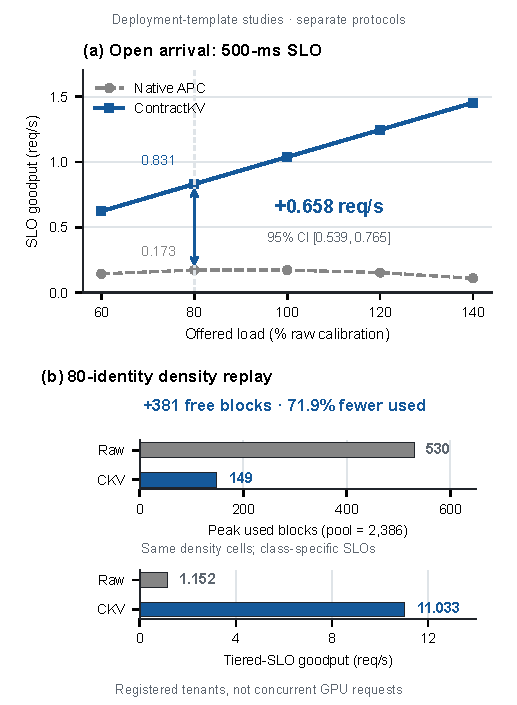
\includegraphics[width=\columnwidth]{figures/fig5_service_goodput_and_kv_savings.pdf}
\caption{Distinct deployment protocols. (a) Open-arrival 500-ms SLO goodput, with the archived hierarchical-bootstrap interval for the absolute increase at 80\% load; 4.81$\times$ is that point's ratio. (b) The same 80-identity density cells supply occupancy and goodput under class-specific 750/1,500/3,000-ms SLOs, with a 2,386-block pool. Registered identities are not simultaneous GPU requests.}
\label{fig:service}
\end{figure}

At 25 tenants/template and 80\% calibrated arrival load, deployment 500-ms goodput rises from 0.173 to 0.831 requests/s: +0.658, with a hierarchical-bootstrap 95\% interval [0.539,0.765] (Fig.~\ref{fig:service}). Across 10--80 registered identities, bounded-concurrency density replay sustains 9.408--11.072 tiered-SLO requests/s versus native APC's 0.900--1.152 (Supplementary Table~S-III). At 80 identities, the same cells use 71.9\% fewer blocks, leaving 381 additional free blocks. They jointly measure consolidation and service benefit without isolating headroom as the sole cause. These marker-bearing deployment traces have a separate task-quality audit from the primary cohort.

\noindent\emph{Finding:} publication governance retains the frozen layout's service benefit, and the template object supports measurable cost sharing and physical consolidation across tenants.


\subsubsection{Physical authorization on every route}
\label{sec:authorization-results}
Authorization must survive raw fallback. Nine fresh-server cells (three models, three repetitions) each exercise six real-task contexts and one marker context without clearing the cache. The 828 business requests comprise 702 real-task and 126 marker controls.

Legacy cross-domain and old-binding/new-epoch raw fallback each hit the prior prefix in 63/63 controls. Domain/epoch-bound block hashes prevent both first-request hits while retaining authorized same-domain sharing (Table~\ref{tab:physical-authorization}). The authority denies all 63 stale identities before dispatch; 93 rejected/abstained qualifications add zero candidate tokens. Physical sharing therefore follows authorization through every route.

\begin{table}[t]
\centering\footnotesize
\setlength{\tabcolsep}{3pt}
\caption{All-route authorization integration, three models and three processes. Each physical check has 63 controls: seven contexts $\times$ nine cells. Repeats share contexts. The engine is not cleared between checks.}
\label{tab:physical-authorization}
\begin{tabular}{@{}P{2.38in}r@{}}
\toprule
Sharing condition & Native hit / controls\\
\midrule
Same domain/epoch, same principal repeat & 63/63\\
Same domain/epoch, second authorized principal & 63/63\\
Different domain, first request & 0/63\\
New active epoch, first request & 0/63\\
New domain/epoch, own subsequent repeat & 63/63 each\\
\bottomrule
\end{tabular}
\end{table}

\subsection{What Determines the Operating Region?}
\label{sec:residency}
\begin{figure}[!t]
\centering
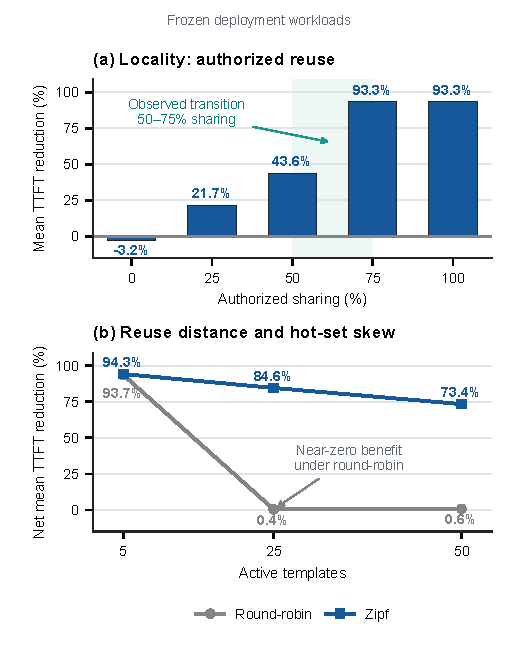
\includegraphics[width=\columnwidth]{figures/fig6_locality_and_residency.pdf}
\caption{Operating region in frozen deployment workloads. (a) The shaded 50--75\% sharing interval is an observed transition, not a universal threshold. (b) Access-pattern sensitivity to reuse distance and hot-set skew. Both axes report TTFT reduction; neither is a direct residency fraction.}
\label{fig:region}
\end{figure}

The object pays off when authorized reuse is sufficiently dense and its physical state remains available. Figure~\ref{fig:region} varies these conditions with a frozen deployment workload. Benefit rises sharply over an observed sharing interval, but round-robin access to a larger working set nearly eliminates it. A qualified object still needs resident physical blocks. In the primary cohort, 189 compiled business requests have incomplete hits: 135 Llama zero hits, 42 Mistral zero hits, and 12 Qwen partial hits. All 1,440 compiled business requests match the certified prefix IDs and commit boundary; each incomplete-hit request has a later full-hit peer in its two-request wave.

Three known-source probes replay archived IDs with read-only lookup/publication/reclamation hooks. Among 138 business requests and four qualifications, all 13 incomplete hits follow deletion of the last matching native mapping at reference count zero; salt/hash chains still match. All 12 immediate post-commit controls hit fully. This diagnoses native reclamation~\cite{vllmAPC} in those sources, not every historical miss or serving performance. Figure~\ref{fig:performance} charges actual recomputation.

\begin{table}[t]
\centering\small
\caption{Four sealed operating points under the development-frozen benefit gate. Net benefit is per certificate; rejected points serve raw. Candidate diagnostics were also run for rejected points, so this table does not measure avoided online verifier calls.}
\label{tab:gate}
\begin{tabular}{@{}rrrrr@{}}
\toprule
Prefix & Uses & Slack (s) & Route & Net benefit (s)\\
\midrule
1500 & 8 & 3.5 & Raw & 0.00\\
3000 & 12 & 0.5 & CKV & 7.04\\
5000 & 10 & 1.5 & CKV & 10.84\\
3500 & 6 & 6 & Raw & 0.00\\
\bottomrule
\end{tabular}
\end{table}


The frozen benefit gate selects two of four sealed points (Table~\ref{tab:gate}); both selected points are net-positive at 7.04 and 10.84 s/certificate. Rejected points serve raw, while their candidate outcomes remain diagnostics. This validates the declared operating-point rule, not a learned predictor or a claim that diagnostic verifier work was avoided.

\paragraph{Sensitivity to input and cost profiles.}\label{sec:costvariant}
\label{sec:fidelity}
The full-cost benefit depends on qualified coverage and faithful inputs. Preserving HotpotQA evidence and RepoBench indentation raises raw HotpotQA F1 from 0 to 0.22222 and raw code score from 0.12067 to 0.36667 in a fixed four-source development comparison; admitted coverage increases from 30/360 to 112/360 and complete-wall throughput from 1.039$\times$ to 1.117$\times$. Those are input-construction, not reordering-induced accuracy gains. A separate length-aware cost-profile variant lowers one Qwen p99 point estimate but sacrifices coverage and throughput; the negative tradeoff and its uncertainty remain in the Supplement.

\noindent\emph{Finding:} scope determines admissible sharing, and locality, residency and admission cost determine how much of that opportunity becomes service benefit.

\subsection{What Does the External Comparator Establish?}
\label{sec:baselines}
The external comparison measures paired task-score changes against each method's native reference. Under the same $>0.03$ reporting threshold, a CacheBlend adapter records 224 decreases and 331 increases in 2,250 pairs against its own separator-matched reference; ContractKV records two decreases and no increases in 2,250 pairs against its own raw APC reference. These reference-relative distributions characterize each adapter; execution stacks and inputs differ. Supplementary Table~S-VIII reports native baselines and threshold sensitivity.

\noindent\emph{Finding:} good average task scores and absence of harmful per-request changes are distinct outcomes; compare them against the actual reference each method uses.
